\documentclass[11pt]{article}
\usepackage[utf8]{inputenc}
\usepackage[czech]{babel}
\usepackage{graphicx}

\title{Krásy počítačové grafiky: Úpravy rastrového obrazu}
\author{Tomáš Maršálek}
\date{9.\,března 2012}

\begin{document}
\maketitle

\section{Zadání}
Vyzkoušejte si naprogramovat metody úpravy digitalizovaného obrazu z přednášky,
jako je ostření, reliéf, warping, morphing.... Za program umějící aspoň jednu
techniku získáte 5 bodů, za každou další naprogramovanou techniku získáte max.
3 body podle obtížnosti, dohromady nejvýše 17 bodů. Program musí být schopen
načíst ze souboru obraz v rastrovém formátu a zase jej uložit, zobrazit původní
a změněný obraz s možností návratu o 1 akci. Odevzdáváte jako obvykle zdrojový
text, EXE a dokumentaci.

\section{Implementované filtry}

\begin{figure}[ht!]
\centering
	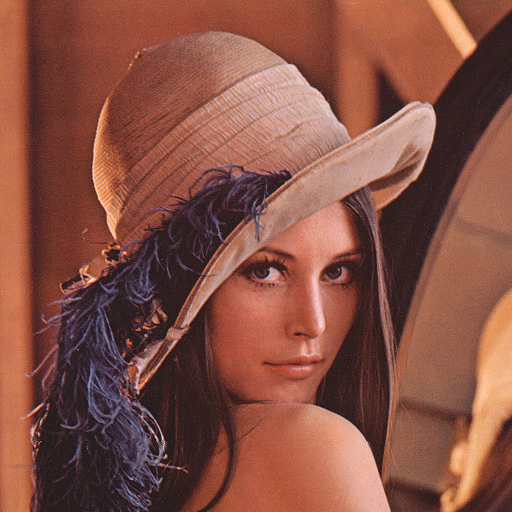
\includegraphics[width=8cm]{lena.png}
	\caption{Originální obrázek}
\end{figure}

\subsection{Detekce hran}
Detekce hran je horní propust pro obrazový signál. Vysokou frekvencí v
rastrovém obrazu se rozumí velký rozdíl v intenzitě barvy v jednotlivých
kanálech.

\subsubsection{Sobel, Prewitt a Roberts Cross}
Jedná se o metody, které pro každý obrazový bod aplikují numerickou aproximaci
první derivace v tomto bodě. Pro dva rozměry se vypočte velikost první derivace
jako velikost gradientu, kde jednotlivé parciální derivace mají své příslušné
konvoluční matice. Vyšší změna barvy se projeví vyšší hodnotou derivace, což
vidíme jako detekovanou hranu. 

Například Sobelův operátor používá konvoluční matice: \\
$$
D_x = 
\left[
\begin{array}{ccc}
-1 & 0 & 1 \\
-2 & 0 & 2 \\
-1 & 0 & 1 \\
\end{array}
\right]
,~~~~
D_y = 
\left[
\begin{array}{ccc}
-1 & -2 & -1 \\
0 & 0 & 0 \\
1 & 2 & 1 \\
\end{array}
\right]
$$

\begin{figure}[ht!]
\centering
	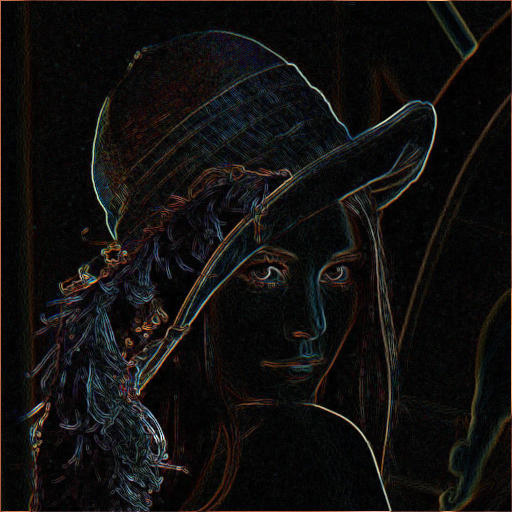
\includegraphics[width=8cm]{sobel.png}
	\caption{Detekce hran, Sobel}
\end{figure}

\subsubsection{Rozdíl Gaussovských rozostření}
Rozostření funguje jako dolní propust pro obrazový signál. Největší změny
oproti původnímu obrázku nastanou právě v místech, kde se nachází hrany. Ty se
relativně rozostří nejvíce. Proto když od původního obrázku odečteme jeho
rozostřenou verzi, největší změnu uvidíme právě v místech hran.

Rozdíl dvou různě silných rozostření je pouze zobecnění rozdílu rozostření s
původním obrázkem.

\begin{figure}[ht!]
\centering
	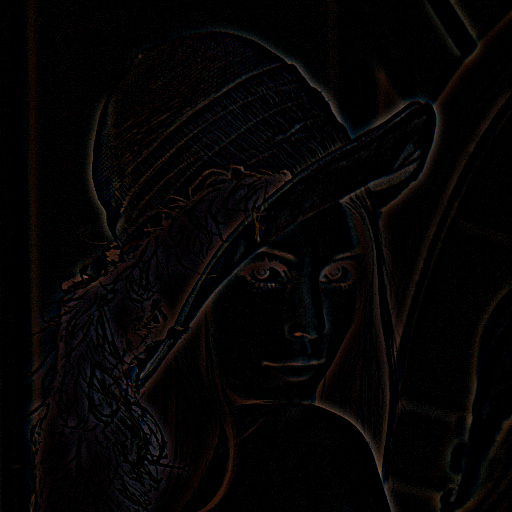
\includegraphics[width=8cm]{difgaus.png}
	\caption{Rozdíl Gaussovských rozostření s variancemi 5 a 0.1}
\end{figure}
\clearpage

\subsubsection{Laplacian of Sobel}
Laplaceův operátor je numerickou aproximací druhé derivace. Aplikací na rastr
získáme velmi tenké hrany, mnohem tenčí, než získané z výše uvedených metod.
Nevýhodou je, že je velmi citlivý na jakýkoliv šum. Proto některé filtry před
použitím Laplaceova operátoru odstraní šum, například Gaussovským rozostřením
(Laplacian of Gaussian) nebo Mediánovým filtrem.

Zde je Laplaceův operátor aplikován po Sobelově operátoru, výsledkem jsou velmi
tenké hrany s minimálním okolním šumem.

\begin{figure}[ht!]
\centering
	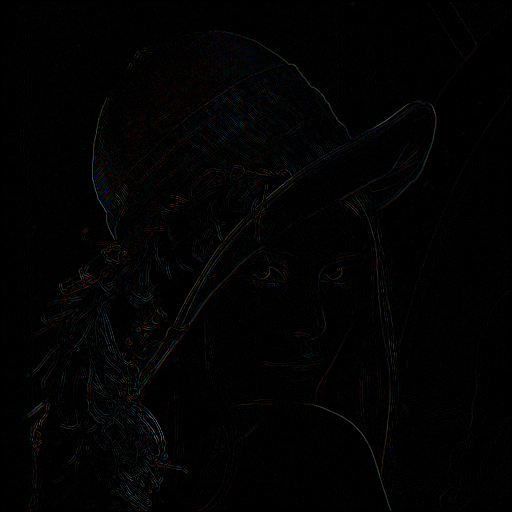
\includegraphics[width=8cm]{los.png}
	\caption{Laplacian of Sobel}
\end{figure}
\clearpage

\subsection{Doostření}
Doostření obrázku je výsledkem součtu původního obrázku s jeho Laplaciánem.
Standardně je implementována možnost měnit intenzitu doostření pomocí
koeficientu ostření. \\

$$
B = A + c \cdot \Delta A
$$
$A$ je původní obrázek, $\Delta$ je Laplaceův operátor, $B$ je doostřený
obrázek a $c$ je koeficient ostření.

\begin{figure}[ht!]
\centering
	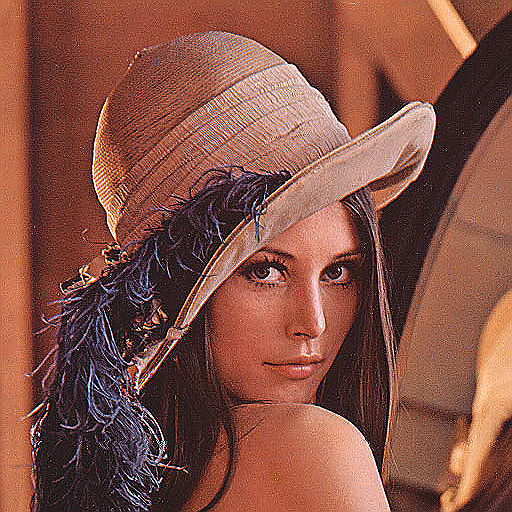
\includegraphics[width=8cm]{sharpen.png}
	\caption{Doostření s koeficientem 5}
\end{figure}


\subsection{Gaussovské rozostření}
Obecně filtr rozostření můžeme chápat jako konvoluci s nějakou průměrující
funkcí. Například standardní rozostření, tzn. průměr okolních bodů je konvoluce
obrázku s dvourozměrnou jednotkovou funkcí. Gaussovské rozostření pouze místo
jednotkové funkce používá Gaussovu křivku jako funkci s koeficienty
průměrování.  

Konvoluce s větší konvoluční maticí je výpočetně náročná operace,
pro každý bod musí provést $k^2$ operací, kde $k$ je velikost strany konvoluční
matice. Při detekci hran tento problém není třeba řešit, protože pracujeme
pouze s maticemi velikosti 3x3. Při standardním nastavení Gaussovského
rozostření však už pracujeme s maticí 16x16, při větších rozptylech pak ještě
mnohem většími, proto je použita známá optimalizace rozdělení konvoluce do
jednotlivých komponent. Dvourozměrná Gaussova funkce je totiž součin dvou
jednorozměrných, využití spočívá v provedení dvou jednorozměrných konvolucí po
sobě, namísto jedné dvourozměrné.

\begin{figure}[ht!]
\centering
	
\includegraphics[width=8cm]{gaus.png}
	\caption{Gaussovské rozostření s variancí 3}
\end{figure}
\clearpage

\subsection{Inverze barev}
Je velmi jednoduchý filtr, ale je zahrnut do programu, aby bylo možné pozorovat
oba způsoby detekce hran: světlé na tmavém pozadí a tmavé na světlém pozadí.
Filtr pouze odečte barvu od maximální hodnoty pro každý pixel.

\begin{figure}[ht!]
\centering
	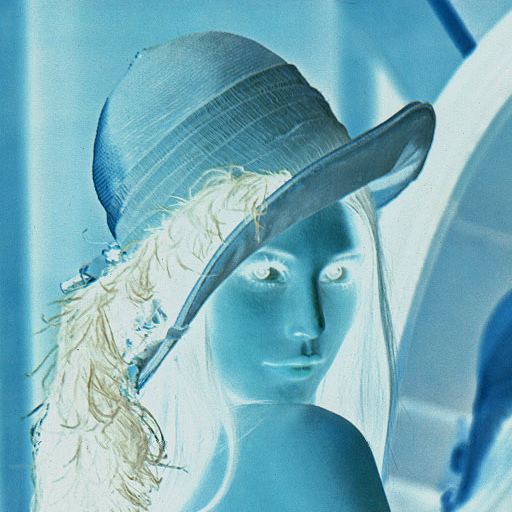
\includegraphics[width=8cm]{invert.png}
	\caption{Inverze barev}
\end{figure}
\clearpage

\subsection{Odbarvení}
Tento filtr je také jednoduchý, ale je zajímavý, protože existuje více způsobů,
jak odbarvení dosáhnout. První je jednoduchý průměr všech tří kanálu. Pro
lidské oko je však kvalitnější volba luminance, protože průměruje kanály
podle vnímání lidského oka ($.2125\cdot R + .7152\cdot G + .0722\cdot B$).

\begin{figure}[ht!]
\centering
	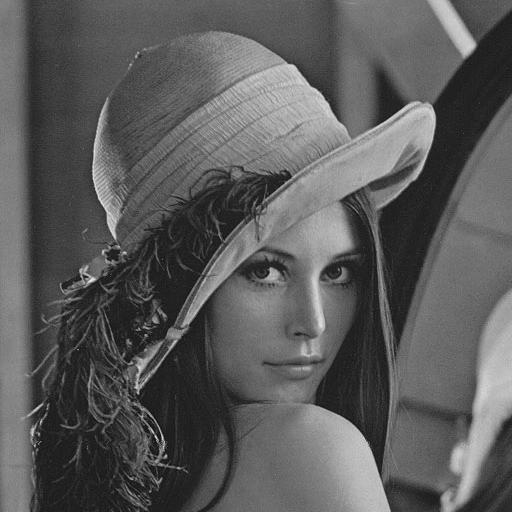
\includegraphics[width=8cm]{luminance.png}
	\caption{Odbarvení pomocí luminance}
\end{figure}

\section{Uživatelské rozhraní}
Grafické rozhraní je vytvořeno pomocí knihovny GTK+ 3.0, proto by měl vzhled
vypadat nativně na jednotlivých operačních systémech.

Uživatel může otevřít obrázek ve formátu .bmp, .jpg nebo .png a uložit ho pod
stejným nebo změněným názvem. Pro možnost porovnání provedených změn je
implementován systém historie zpět a vpřed. Kromě těchto základních funkcí je
uživateli umožněno používat výše zmíněné filtry, další funkcionalita není
implementována.

\section{Implementace}
Jazyk programu je ANSI C, použitá knihovna grafického prostředí je GTK+ 3.0 a
Glade 3.

Pro spuštění programu musí být ve stejném adresáři přítomen soubor s
uživatelským rozhraním upravovac.glade.

\begin{figure}[ht!]
\centering
	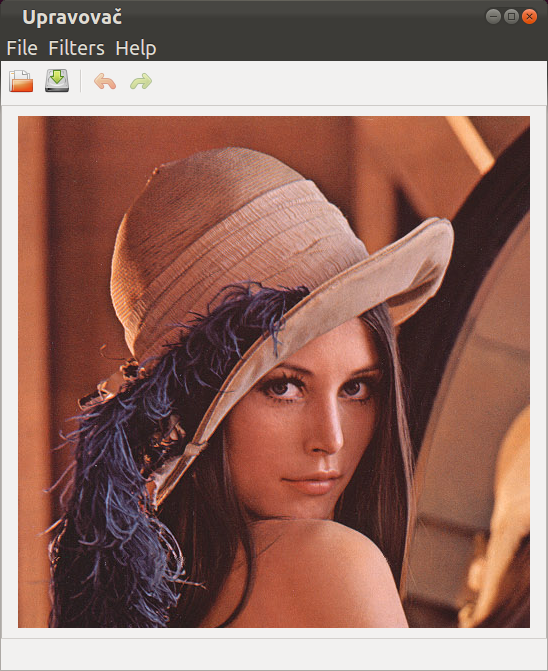
\includegraphics[width=8cm]{gui.png}
	\caption{Ukázka uživatelského rozhraní}
\end{figure}

\section{Závěr}
Tento program má velký potenciál na další úpravy, především v uživatelském
rozhraní a dalších filtrech. Nicméně v takovéto podobě by měl splňovat uvedené
zadání.

\end{document}
